\documentclass[11pt]{article}
\usepackage{amsmath}
\usepackage{amssymb}
\usepackage{graphicx}
\usepackage{tabularx}
\usepackage{fancyhdr}
\usepackage{lastpage}

% Page layout
\usepackage[top=1in, bottom=1in, left=1in, right=1in]{geometry}

% Header and footer
\pagestyle{fancy}
\fancyhf{}
\rfoot{Page \thepage}
\renewcommand{\headrulewidth}{0pt}

% Modified Question command with left-aligned number
\newcommand{\questiona}[2]{
    \noindent\textbf{Q#2.} #1 \hfill \textbf{[1 Mark]}
}

\newcommand{\questionb}[2]{
    \noindent\textbf{Q#2.} #1 \hfill \textbf{[2 Marks]}
}

\begin{document}

% Title section with horizontal line
\begin{center}
    \Large\textbf{GATE 2018 - Aerospace Engineering (ECE)} \\
    \large\textbf{General Aptitude and Technical Questions} \\
    \rule{\textwidth}{0.5pt} % Horizontal line below heading
\end{center}

\vspace{0.5cm}

% General Aptitude Section
\section*{General Aptitude}

\questiona{The dress \_\_\_\_\_ her so well that they all immediately \_\_\_\_\_ her on her appearance.}{1}
\begin{enumerate}
    \item[(A)] complemented, complemented  
    \item[(B)] complimented, complemented  
    \item[(C)] complimented, complimented  
    \item[(D)] complemented, complimented  
\end{enumerate}

\vspace{0.5cm}

\questiona{The judge’s standing in the legal community, though shaken by false allegations of wrongdoing, remained \_\_\_\_\_.}{2}
\begin{enumerate}
    \item[(A)] undiminished  
    \item[(B)] damaged  
    \item[(C)] illegal  
    \item[(D)] uncertain  
\end{enumerate}

\vspace{0.5cm}

\questiona{Find the missing group of letters in the following series: BC, FGH, LMNO, \_\_\_\_\_}{3}
\begin{enumerate}
    \item[(A)] UVWXY  
    \item[(B)] TUVWX  
    \item[(C)] STUVW  
    \item[(D)] RSTUV  
\end{enumerate}

\vspace{0.5cm}

\questiona{The perimeters of a circle, a square and an equilateral triangle are equal. Which one of the following statements is true?}{4}
\begin{enumerate}
    \item[(A)] The circle has the largest area.  
    \item[(B)] The square has the largest area.  
    \item[(C)] The equilateral triangle has the largest area.  
    \item[(D)] All the three shapes have the same area.  
\end{enumerate}

\vspace{0.5cm}

\questiona{The value of the expression $\frac{1}{1+\log_u vw} + \frac{1}{1+\log_v wu} + \frac{1}{1+\log_w uv}$ is \_\_\_\_\_.}{5}
\begin{enumerate}
    \item[(A)] $-1$  
    \item[(B)] $0$  
    \item[(C)] $1$  
    \item[(D)] $3$  
\end{enumerate}

\vspace{0.5cm}

\questionb{Forty students watched films A, B and C over a week. Each student watched either only one film or all three. Thirteen students watched film A, sixteen students watched film B and nineteen students watched film C. How many students watched all three films?}{6}
\begin{enumerate}
    \item[(A)] 0  
    \item[(B)] 2  
    \item[(C)] 4  
    \item[(D)] 8  
\end{enumerate}

\vspace{0.5cm}

\questionb{A wire would enclose an area of 1936 m\textsuperscript{2}, if it is bent into a square. The wire is cut into two pieces. The longer piece is thrice as long as the shorter piece. The long and the short pieces are bent into a square and a circle, respectively. Which of the following choices is closest to the sum of the areas enclosed by the two pieces in square meters?}{7}
\begin{enumerate}
    \item[(A)] 1096  
    \item[(B)] 1111  
    \item[(C)] 1243  
    \item[(D)] 2486  
\end{enumerate}

\vspace{0.5cm}

\questionb{A contract is to be completed in 52 days and 125 identical robots were employed, each operational for 7 hours a day. After 39 days, five-seventh of the work was completed. How many additional robots would be required to complete the work on time, if each robot is now operational for 8 hours a day?}{8}
% No options since marks were awarded to all

\vspace{0.5cm}

\questionb{A house has a number which needs to be identified. The following three statements are given that can help in identifying the house number.

\begin{itemize}
    \item If the house number is a multiple of 3, then it is a number from 50 to 59.
    \item If the house number is NOT a multiple of 4, then it is a number from 60 to 69.
    \item If the house number is NOT a multiple of 6, then it is a number from 70 to 79.
\end{itemize}

What is the house number?}{9}
\begin{enumerate}
    \item[(A)] 54  
    \item[(B)] 65  
    \item[(C)] 66  
    \item[(D)] 76  
\end{enumerate}

\vspace{0.5cm}

\questionb{An unbiased coin is tossed six times in a row and four different such trials are conducted. One trial implies six tosses of the coin. If H stands for head and T stands for tail, the following are the observations from the four trials:

\begin{itemize}
    \item (1) HTHTHT
    \item (2) TTHHHT
    \item (3) HTTHHT
    \item (4) HHHT\_\_\_\_
\end{itemize}

Which statement describing the last two coin tosses of the fourth trial has the highest probability of being correct?}{10}
\begin{enumerate}
    \item[(A)] Two T will occur.  
    \item[(B)] One H and one T will occur.  
    \item[(C)] Two H will occur.  
    \item[(D)] One H will be followed by one T.  
\end{enumerate}

\vspace{0.8cm}

\section*{Technical Section}

\questiona{Let $\vec{a}, \vec{b}$ be two distinct vectors that are not parallel. The vector $c = \vec{a} \times \vec{b}$ is}{1}
\begin{enumerate}
    \item[(A)] zero  
    \item[(B)] orthogonal to $\vec{a}$ alone  
    \item[(C)] orthogonal to $\vec{a} + \vec{b}$  
    \item[(D)] orthogonal to $\vec{b}$ alone  
\end{enumerate}

\vspace{0.5cm}

\questiona{Consider the function $f(x, y) = \frac{x^2}{2} + \frac{y^2}{3} - 5$. All the roots of this function}{2}
\begin{enumerate}
    \item[(A)] form a finite set of points  
    \item[(B)] lie on an elliptical curve  
    \item[(C)] lie on the surface of a sphere  
    \item[(D)] lie on a hyperbolic curve  
\end{enumerate}

\vspace{0.5cm}

\questiona{Consider a vector field given by $x\hat{i} + y\hat{j} + z\hat{k}$. This vector field is}{3}
\begin{enumerate}
    \item[(A)] divergence-free and curl-free  
    \item[(B)] curl-free but not divergence-free  
    \item[(C)] divergence-free but not curl-free  
    \item[(D)] neither divergence-free nor curl-free  
\end{enumerate}

\vspace{0.5cm}

\questiona{A jet aircraft is initially flying steady and level at its maximum endurance condition. For the aircraft to fly steady and level, but faster at the same altitude, the pilot should}{4}
\begin{enumerate}
    \item[(A)] increase thrust alone  
    \item[(B)] increase thrust and increase angle of attack  
    \item[(C)] increase thrust and reduce angle of attack  
    \item[(D)] reduce angle of attack alone  
\end{enumerate}

\vspace{0.5cm}

\questiona{The pilot of a conventional airplane that is flying steady and level at some altitude, deflects the port side aileron up and the starboard aileron down. The aircraft will then}{5}
\begin{enumerate}
    \item[(A)] pitch, nose up  
    \item[(B)] roll with the starboard wing up  
    \item[(C)] pitch, nose down  
    \item[(D)] roll with the port wing up  
\end{enumerate}

\vspace{0.5cm}

\questiona{A NACA 0012 airfoil has a trailing edge flap. The airfoil is operating at an angle of attack of $5^\circ$ with un-deflected flap. If the flap is now deflected by $5^\circ$ downwards, the $C_L$ versus $\alpha$ curve}{6}
\begin{enumerate}
    \item[(A)] shifts right and slope increases  
    \item[(B)] shifts left and slope increases  
    \item[(C)] shifts left and slope stays the same  
    \item[(D)] shifts right and slope stays the same  
\end{enumerate}

\vspace{0.5cm}

\questiona{An airplane requires a longer ground roll to lift-off on hot summer days because}{7}
\begin{enumerate}
    \item[(A)] the thrust is directly proportional to free-stream density  
    \item[(B)] the thrust is directly proportional to weight of the aircraft  
    \item[(C)] the lift-off distance is directly proportional to free-stream density  
    \item[(D)] the runway friction is high on hot summer days  
\end{enumerate}

\vspace{0.5cm}

\questiona{The velocity profile in an incompressible, laminar boundary layer is shown in the figure below. $U$ is the free-stream velocity, $u(y)$ is the stream-wise velocity component. The area of the black shaded region in the figure represents the}{8}

\begin{center}
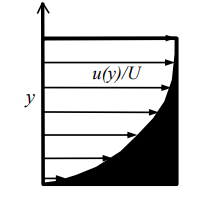
\includegraphics[width=0.5\textwidth]{figures/8.png}
\end{center}

\begin{enumerate}
    \item[(A)] boundary layer thickness  
    \item[(B)] momentum thickness  
    \item[(C)] displacement thickness  
    \item[(D)] shape factor  
\end{enumerate}

\vspace{0.5cm}

\questiona{The tangential velocity component $V$ of a spacecraft, which is in a circular orbit of radius $R$ around a spherical Earth ($\mu = GM$ gravitational parameter of Earth) is given by the following expression.}{9}
\begin{enumerate}
    \item[(A)] $V = \sqrt{\frac{\mu}{2R}}$  
    \item[(B)] $V = \sqrt{\frac{\mu}{R}}$  
    \item[(C)] $V = \frac{2\pi}{\sqrt{\mu}} R^{3/2}$  
    \item[(D)] $V = \frac{2\pi}{\sqrt{\mu}} R^{2/3}$  
\end{enumerate}

\vspace{0.5cm}

\questiona{Equation of the trajectory of a typical space object around any planet, in polar coordinates $(r, \theta)$ is given as follows (where $h$ is angular momentum, $\mu$ is gravitational parameter, $e$ is eccentricity):}{10}
\begin{enumerate}
    \item[(A)] $r = \frac{h^2/\mu}{1 - e\cos\theta}$  
    \item[(B)] $r = \frac{h^2/\mu}{e - \cos\theta}$  
    \item[(C)] $r = \frac{h^2/\mu}{1 + e\cos\theta}$  
    \item[(D)] $r = \frac{h^2/\mu}{e + \cos\theta}$  
\end{enumerate}

\vspace{0.5cm}

\questiona{In an elliptic orbit around any planet, the location at which a spacecraft has the maximum angular velocity is}{11}
\begin{enumerate}
    \item[(A)] apoapsis  
    \item[(B)] periapsis  
    \item[(C)] a point at $+45^\circ$ from periapsis  
    \item[(D)] a point at $-90^\circ$ from apoapsis  
\end{enumerate}

\vspace{0.5cm}

\questiona{The pitching moment of a positively cambered NACA airfoil about its leading edge at zero-lift angle of attack is}{12}
\begin{enumerate}
    \item[(A)] negative  
    \item[(B)] positive  
    \item[(C)] indeterminate  
    \item[(D)] zero  
\end{enumerate}

\vspace{0.5cm}

\questiona{In a low-speed wind tunnel, the angular location(s) from the front stagnation point on a circular cylinder where the static pressure equals the free-stream static pressure, is}{13}
\begin{enumerate}
    \item[(A)] $\pm 38^\circ$  
    \item[(B)] $\pm 30^\circ$  
    \item[(C)] $\pm 60^\circ$  
    \item[(D)] $0^\circ$  
\end{enumerate}

\vspace{0.5cm}

\questiona{A thermocouple, mounted flush in an insulated flat surface in a supersonic laminar flow of air measures the}{14}
\begin{enumerate}
    \item[(A)] static temperature  
    \item[(B)] temperature greater than static but less than total temperature  
    \item[(C)] total temperature  
    \item[(D)] temperature greater than total temperature  
\end{enumerate}

\vspace{0.5cm}

\questiona{A shock wave is moving into still air in a shock tube. Which one of the following happens to the air?}{15}
\begin{enumerate}
    \item[(A)] static temperature increases, total temperature remains constant  
    \item[(B)] static temperature increases, total temperature increases  
    \item[(C)] static temperature increases, total temperature decreases  
    \item[(D)] static pressure increases, total temperature remains constant  
\end{enumerate}

\vspace{0.5cm}

\questiona{The highest limit load factor experienced by a civil transport aircraft is in the range}{16}
\begin{enumerate}
    \item[(A)] 0.0 -- 2.0  
    \item[(B)] 2.0 -- 5.0  
    \item[(C)] 5.0 -- 8.0  
    \item[(D)] 8.0 -- 10.0  
\end{enumerate}

\vspace{0.5cm}

\questiona{Determine the correctness or otherwise of the following statements, [a] and [r]: 

\(a\) A closed-section box beam configuration is used in aircraft wings. \\
\(r\) Closed-section box beam configuration is capable of resisting torsional loads.}{17}
\begin{enumerate}
    \item[(A)] Both [a] and [r] are true and [r] is the correct reason for [a]  
    \item[(B)] Both [a] and [r] are true but [r] is not the correct reason for [a]  
    \item[(C)] Both [a] and [r] are false  
    \item[(D)] [a] is true but [r] is false  
\end{enumerate}

\vspace{0.5cm}

\questiona{The first law of thermodynamics is also known as conservation of}{18}
\begin{enumerate}
    \item[(A)] mass  
    \item[(B)] momentum  
    \item[(C)] energy  
    \item[(D)] species  
\end{enumerate}

\vspace{0.5cm}

\questiona{In an ideal gas turbine cycle, the expansion in a turbine is represented by}{19}
\begin{enumerate}
    \item[(A)] an isenthalpic process  
    \item[(B)] an isentropic process  
    \item[(C)] an isobaric process  
    \item[(D)] an isochoric process  
\end{enumerate}

\vspace{0.5cm}

\questiona{The determinant of the matrix $\begin{bmatrix} 1 & 1 & -1 \\ 2 & 1 & 0 \\ 3 & 1 & 1 \end{bmatrix}$ is \_\_\_\_\_ (accurate to one decimal place).}{20}

\vspace{0.5cm}

\questiona{The theoretical maximum velocity (in m/s) of air expanding from a reservoir at 700 K is \_\_\_\_\_ (accurate to two decimal places). Specific heat of air at constant pressure is 1005 J/(kg-K).}{21}

\vspace{0.5cm}

\questiona{For a damped single degree of freedom system with damping ratio of 0.1, ratio of two successive peak amplitudes of free vibration is \_\_\_\_\_ (accurate to two decimal places).}{22}

\vspace{0.5cm}

\questiona{The natural frequency (in rad/s) of the spring-mass system shown in the figure below is \_\_\_\_\_ (accurate to one decimal place).}{23}
\begin{center}
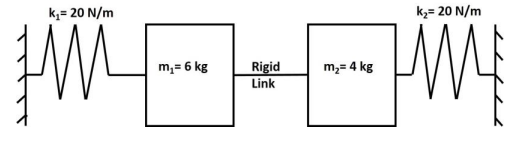
\includegraphics[width=0.5\textwidth]{figures/23.png}
\end{center}

\vspace{0.5cm}

\questiona{The stagnation pressures at the inlet and exit of a subsonic intake are 100 kPa and 98 kPa, respectively. The pressure recovery of this intake will be \_\_\_\_\_ (accurate to two decimal places).}{24}

\vspace{0.5cm}

\questiona{A combustor is operating with a fuel-air ratio of 0.03. If the stoichiometric fuel-air ratio of the fuel used is 0.06, the equivalence ratio of the combustor will be \_\_\_\_\_ (accurate to two decimal places).}{25}

\vspace{0.5cm}

% Technical Questions Continued
\section*{Technical (Aerospace Engineering) -- Continued}

\questionb{The solution of the differential equation $\frac{d^2y}{dx^2} + 3\frac{dy}{dx} = 0$, given that $y = 0$ and $\frac{dy}{dx} = 1$ at $x = 0$ is}{26}
\begin{enumerate}
    \item[(A)] $x(1 - e^{-3x})$  
    \item[(B)] $\frac{1}{3}(1 - e^{-3x})$  
    \item[(C)] $\frac{1}{3}(1 + e^{-3x})$  
    \item[(D)] $\frac{1}{3}xe^{-3x}$  
\end{enumerate}

\vspace{0.5cm}

\questionb{The relation between pressure ($p$) and velocity ($V$) for a steady, isentropic flow at two points along a streamline is, ($c$ is a constant)}{27}
\begin{enumerate}
    \item[(A)] $c(p_2^{\gamma} - p_1^{\gamma}) = \frac{V_1^2}{2} - \frac{V_2^2}{2}$  
    \item[(B)] $c(p_2^{\frac{\gamma}{\gamma-1}} - p_1^{\frac{\gamma}{\gamma-1}}) = \frac{V_1^2}{2} - \frac{V_2^2}{2}$  
    \item[(C)] $c(p_2^{\frac{\gamma - 1}{\gamma}} - p_1^{\frac{\gamma - 1}{\gamma}}) = \frac{V_1^2}{2} - \frac{V_2^2}{2}$  
    \item[(D)] $c(p_2^{\gamma - 1} - p_1^{\gamma - 1}) = \frac{V_1^2}{2} - \frac{V_2^2}{2}$  
\end{enumerate}

\vspace{0.5cm}

\questionb{A thin airfoil is mounted in a low-speed, subsonic wind tunnel, in which the Mach number is 0.1. At a point on the airfoil, the pressure coefficient is measured to be $-1.2$. If the flow velocity is increased such that the free-stream Mach number is 0.6, the pressure coefficient at the same point on the airfoil will approximately be:}{28}
\begin{enumerate}
    \item[(A)] $-3.5$  
    \item[(B)] $-2.9$  
    \item[(C)] $-1.5$  
    \item[(D)] $-0.75$  
\end{enumerate}

\vspace{0.5cm}

\questionb{A solid circular shaft of diameter $d$ is under pure torsion of magnitude $T$. The maximum tensile stress experienced at any point on the shaft is}{29}
\begin{enumerate}
    \item[(A)] $\frac{32T}{\pi d^3}$  
    \item[(B)] $\frac{16T}{\pi d^4}$  
    \item[(C)] $\frac{32T}{\pi d^4}$  
    \item[(D)] $\frac{16T}{\pi d^3}$  
\end{enumerate}

\vspace{0.5cm}

\questionb{A clamped-clamped beam, subjected to a point load $P$ at the midspan, is shown in the figure below. The magnitude of the moment reaction at the two fixed ends of the beam is}{30}

\begin{center}
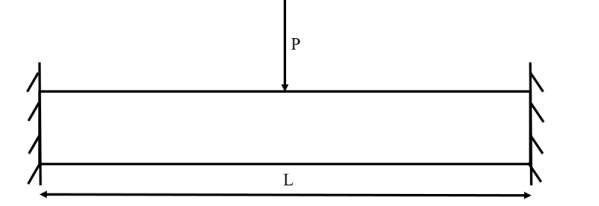
\includegraphics[width=0.5\textwidth]{figures/30.png}
\end{center}

\begin{enumerate}
    \item[(A)] $PL/2$  
    \item[(B)] $PL/4$  
    \item[(C)] $PL/8$  
    \item[(D)] $PL/16$  
\end{enumerate}

\vspace{0.5cm}

\questionb{Which of the following statement(s) is/are true about the state of a body in plane strain condition? \\
P: All the points in the body undergo displacements in one plane only, for example the x-y plane, leading to $\varepsilon_{zz} = \gamma_{xz} = \gamma_{yz} = 0$. \\
Q: All the components of stress perpendicular to the plane of deformation, for example the x-y plane, of the body are equal to zero, i.e. $\sigma_{zz} = \tau_{xz} = \tau_{yz} = 0$. \\
R: Except the normal component, all the other components of stress perpendicular to the plane of deformation of the body, for example the x-y plane, are equal to zero, i.e. $\sigma_{zz} \ne 0, \tau_{xz} = \tau_{yz} = 0$.}{31}
\begin{enumerate}
    \item[(A)] P only  
    \item[(B)] Q only  
    \item[(C)] P and Q  
    \item[(D)] P and R  
\end{enumerate}

\vspace{0.5cm}

\questionb{An aircraft with a turbojet engine flies at a velocity of 100 m/s. If the jet exhaust velocity is 300 m/s, the propulsive efficiency of the engine, assuming a negligible fuel-air ratio, is}{32}
\begin{enumerate}
    \item[(A)] 0.33  
    \item[(B)] 0.50  
    \item[(C)] 0.67  
    \item[(D)] 0.80  
\end{enumerate}

\vspace{0.5cm}

\questionb{An aircraft with a turboprop engine produces a thrust of 500 N and flies at 100 m/s. If the propeller efficiency is 0.5, the shaft power produced by the engine is}{33}
\begin{enumerate}
    \item[(A)] 50 kW  
    \item[(B)] 100 kW  
    \item[(C)] 125 kW  
    \item[(D)] 500 kW  
\end{enumerate}

\vspace{0.5cm}

\questionb{An axial compressor that generates a stagnation pressure ratio of 4.0, operates with inlet and exit stagnation temperatures of 300 K and 480 K, respectively. If the ratio of specific heats ($\gamma$) is 1.4, the isentropic efficiency of the compressor is}{34}
\begin{enumerate}
    \item[(A)] 0.94  
    \item[(B)] 0.81  
    \item[(C)] 0.72  
    \item[(D)] 0.63  
\end{enumerate}

\vspace{0.5cm}

\questionb{A rocket has an initial mass of 150 kg. After operating for a duration of 10 s, its final mass is 50 kg. If the acceleration due to gravity is 9.81 m/s\textsuperscript{2} and the thrust produced by the rocket is 19.62 kN, the specific impulse of the rocket is}{35}
\begin{enumerate}
    \item[(A)] 400 s  
    \item[(B)] 300 s  
    \item[(C)] 200 s  
    \item[(D)] 100 s  
\end{enumerate}

\vspace{0.5cm}

\questionb{Consider the vector field $\vec{F} = -\frac{y}{r^2} \hat{i} + \frac{x}{r^2} \hat{j}$ where $r = \sqrt{x^2 + y^2}$. The contour integral $\oint \vec{F} \cdot d\vec{s}$, where $d\vec{s}$ is tangent to the contour that encloses the origin, is \_\_\_\_\_ (accurate to two decimal places).}{36}

\vspace{0.5cm}

\questionb{The magnitude of the x-component of a unit vector at the point (1, 1) that is normal to equi-potential lines of the potential function $\phi(r) = \frac{1}{r^2 + 4}$, where $r = \sqrt{x^2 + y^2}$, is \_\_\_\_\_ (accurate to two decimal places).}{37}

\vspace{0.5cm}

\questionb{Assuming ISA standard sea level conditions (288.16 K, density of 1.225 kg/m\textsuperscript{3}, $g = 9.81$ m/s\textsuperscript{2}, $R = 287$ J/(kg-K)), the density (in kg/m\textsuperscript{3}) of air at Leh, which is at an altitude of 3500 m above mean sea level is \_\_\_\_\_ (accurate to two decimal places).}{38}

\vspace{0.5cm}

\questionb{Consider a cubical tank of side 2 m with its top open. It is filled with water up to a height of 1 m. Assuming the density of water to be 1000 kg/m\textsuperscript{3}, $g = 9.81$ m/s\textsuperscript{2} and the atmospheric pressure to be 100 kPa, the net hydrostatic force (in kN) on the side face of the tank due to the air and water is \_\_\_\_\_ (accurate to two decimal places).}{39}

\vspace{0.5cm}

\questionb{An aircraft with mass of 400,000 kg cruises at 240 m/s at an altitude of 10 km. Its lift to drag ratio at cruise is 15. Assuming $g = 9.81$ m/s\textsuperscript{2}, the power (in MW) needed for it to cruise is \_\_\_\_\_ (accurate to two decimal places).}{40}

\vspace{0.5cm}

\questionb{A statically-stable aircraft has a $C_{L\alpha} = 5$ (where the angle of attack, $\alpha$, is measured in radians). The coefficient of moment of the aircraft about the center of gravity is given as $C_{M,c.g} = 0.05 - 4\alpha$. The mean aerodynamic chord of the aircraft wing is 1 m. The location (positive towards the nose) of the neutral point of the aircraft from the center of gravity is \_\_\_\_\_ (in m, accurate to two decimal places).}{41}

\vspace{0.5cm}

\questionb{An aircraft with a gross weight of 2000 kg, has a speed of 130 m/s at sea level, where the conditions are: 1 atmosphere (pressure), 288 K (temperature), and 1.23 kg/m\textsuperscript{3} (density). The speed (in m/s) required by the aircraft at an altitude of 9000 m, where the conditions are: 0.31 atmosphere, 230 K, and 0.47 kg/m\textsuperscript{3}, to maintain a steady, level flight is \_\_\_\_\_ (accurate to two decimal places).}{42}

\vspace{0.5cm}

\questionb{A pitot probe on an aircraft in a steady, level flight records a pressure of 55,000 N/m\textsuperscript{2}. The static pressure and density are 45,280 N/m\textsuperscript{2} and 0.6 kg/m\textsuperscript{3}, respectively. The wing area and the lift coefficient are 16 m\textsuperscript{2} and 2, respectively. The wing loading (in N/m\textsuperscript{2}) on this aircraft is \_\_\_\_\_ (accurate to one decimal place).}{43}

\vspace{0.5cm}

\questionb{A spacecraft forms a circular orbit at an altitude of 150 km above the surface of a spherical Earth. Assuming the gravitational parameter, $\mu = 3.986 \times 10^{14}$ m\textsuperscript{3}/s\textsuperscript{2} and radius of Earth, $R_E = 6400$ km, the velocity required for the injection of the spacecraft, parallel to the local horizon, is \_\_\_\_\_ (accurate to two decimal places).}{44}

\vspace{0.5cm}

\questionb{Air at 50 kPa pressure and 400 K temperature flows in a duct at Mach 3.0. A part of the flow leaks through an opening on the duct wall into the ambient, where the pressure is 30 kPa. The maximum Mach number achieved in the discharge is \_\_\_\_\_ (accurate to two decimal places). (Ratio of specific heats of air is $\gamma = 1.4$)}{45}

\vspace{0.5cm}

\questionb{Consider a $20^\circ$ half-angle wedge in a supersonic flow at Mach 3.0 at standard sea-level conditions. If the shock-wave angle on the wedge is $36^\circ$, the Mach number of the tangential component of the flow post-shock is \_\_\_\_\_ (accurate to two decimal places).}{46}

\vspace{0.5cm}

\questionb{The boundary layer thickness at the location of a sensor on a flat plate in an incompressible, laminar flow of air is required to be restricted to 1 mm for an effective measurement. If the flow velocity is 20 m/s with 1 bar pressure, 300 K temperature, and $1.789 \times 10^{-5}$ kg/(m·s) viscosity, the maximum distance (in mm) of the sensor location from the leading edge is \_\_\_\_\_ (accurate to one decimal place).}{47}

\vspace{0.5cm}

\questionb{Gross weight of an airplane is 7000 N, wing area is 16 m\textsuperscript{2}, and the maximum lift coefficient is 2.0. Assuming density at the altitude as 1.23 kg/m\textsuperscript{3}, the stall speed (in m/s) of the aircraft is \_\_\_\_\_ (accurate to two decimal places).}{48}


\vspace{0.5cm}

\questionb{A thin-walled tube with external radius of 100 mm and wall thickness of 2 mm, is fixed at one end. It is subjected to a compressive force of 1 N acting at a point on the circumference parallel to its length. The maximum normal stress (in kPa) experienced by the structure is \_\_\_\_\_ (accurate to two decimal places).}{49}

\vspace{0.5cm}

\questionb{A 1 m long massless cantilever beam oscillates at 2 Hz, while a 60 kg mass is attached at the tip of it. The flexural rigidity of the beam (in kN·m\textsuperscript{2}) is \_\_\_\_\_ (accurate to two decimal places).}{50}

\vspace{0.5cm}

\questionb{A cantilever beam having a rectangular cross-section of width 60 mm and depth 100 mm, is made of aluminum alloy. The material mechanical properties are: Young’s modulus, $E = 73$ GPa and ultimate stress, $\sigma_u = 480$ MPa. Assuming a factor of safety of 4, the maximum bending moment (in kN·m) that can be applied on the beam is \_\_\_\_\_ (accurate to one decimal place).}{51}

\vspace{0.5cm}

\questionb{The components of stress in a body under plane stress condition, in the absence of body forces, is given by: \\
$\sigma_{xx} = Ax^2$, \\
$\sigma_{yy} = 12x^2 - 6y^2$, \\
$\sigma_{xy} = 12xy$. \\
The coefficient $A$, such that the body is under equilibrium, is \_\_\_\_\_ (accurate to one decimal place).}{52}

\vspace{0.5cm}

\questionb{An axial compressor rotor with 50\% degree of reaction operates with an axial velocity of 200 m/s. The absolute flow angle at the inlet of the rotor is $22^\circ$ with reference to the axial direction. If the axial velocity is assumed to remain constant through the rotor, the magnitude of the relative velocity (in m/s) at the rotor exit is \_\_\_\_\_ (accurate to one decimal place).}{53}

\vspace{0.5cm}

\questionb{The relative velocity of air leaving a straight radial impeller of a centrifugal compressor is 100 m/s. If the impeller tip speed is 200 m/s, for a slip-free operation, the absolute velocity (in m/s) at the impeller exit is \_\_\_\_\_ (accurate to one decimal place).}{54}

\vspace{0.5cm}

\questionb{An aircraft wind tunnel model, having a pitch axis mass moment of inertia ($I_{yy}$) of 0.014 kg·m\textsuperscript{2}, is mounted in such a manner that it has pure pitching motion about its center of gravity, where it is supported through a frictionless hinge. If the pitching moment ($M$) derivative with respect to angle of attack ($\alpha$), denoted by $M_\alpha$, is -0.504 N·m/rad and the pitching moment ($M$) derivative with respect to pitch rate ($q$), denoted by $M_q$, is -0.0336 N·m/(rad/s), the damping ratio of the resulting motion due to an initial disturbance in pitch angle is approximately \_\_\_\_\_ (accurate to three decimal places).}{55}

\vspace{0.5cm}




\vspace{5cm}
\begin{center}
\textbf{END OF THE QUESTION PAPER}
\rule{\textwidth}{0.5pt} 
\end{center}

\end{document}
